\documentclass{article}
\usepackage{titling}
\usepackage{graphicx}
\usepackage{indentfirst}
\usepackage{amsmath}
\usepackage{float}
\usepackage[a4paper, total={6in, 10in}]{geometry}
\graphicspath{ {images/} }

\title{Dungeon Report}
\author{109550059 Yen-chieh Huang\thanks{I cannot type in my Chinese name in \LaTeX{} :(}}
\predate{}
\postdate{}
\date{}

\begin{document}

\maketitle
\tableofcontents
\newpage

\section{Implementation Detail}

    \subsection{Class Hierarchy}
    
    \begin{figure}[h]
        \centering
        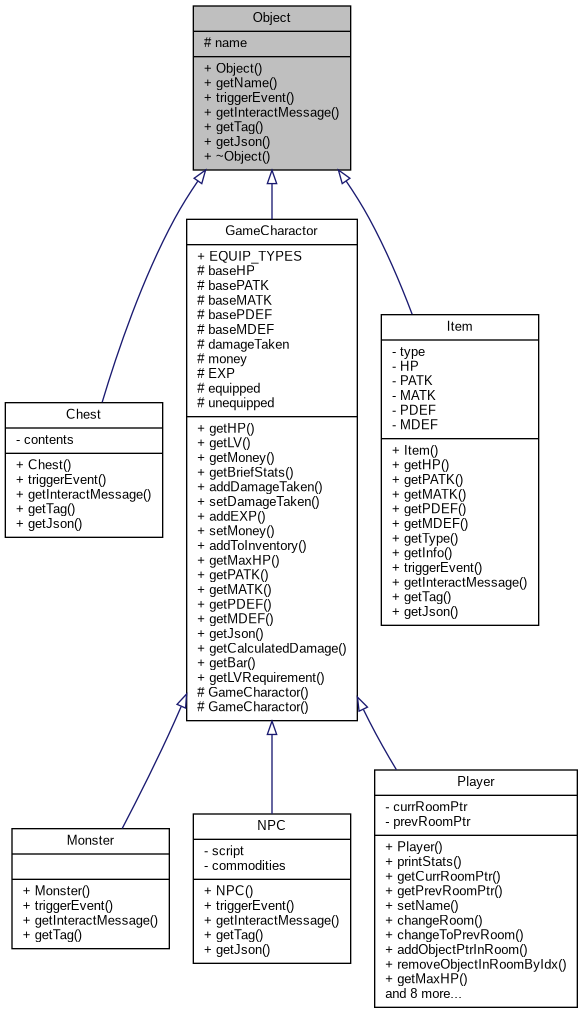
\includegraphics[width=0.6\linewidth]{object_uml}
        \caption{Object's UML Diagram}
    \end{figure}
    \begin{figure}
        \begin{center}
            \begin{minipage}[c]{0.4\linewidth}
                \begin{center}
                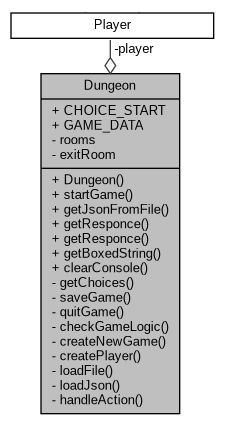
\includegraphics[width=0.7\linewidth]{dungeon_uml}
                \end{center}
                \caption{Dungeon's UML Diagram}
            \end{minipage}
            \text{     }
            \begin{minipage}[c]{0.4\linewidth}
                \begin{center}
                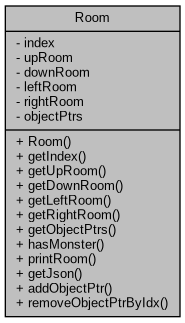
\includegraphics[width=0.7\linewidth]{room_uml}
                \end{center}
                \caption{Room's UML Diagram}
            \end{minipage}
        \end{center}
    \end{figure}
    
    \subsection{Actions Menu}
    The actions menu is implemented by checking whether the room is connected to other room, and then loop through all objects in the room (by calling virtual function \texttt{getInteractMessage()}). If there are monsters in the room, then all the rooms except the previous one are locked. In this case, the only movement player can make is retreat. Each action is assigned with a special character (e.g. \textit{a} represents moving to the left room, \textit{1} might be talking to NPC).
    \par
    Once the program printed out all the actions available, it then prompt user to input a character. If user input \textit{w}, \textit{a}, \textit{s}, or \textit{d}, the player will move to its corresponding room. If user input \textit{e}, player's stats and inventory will be printed out. If the input is a numeric value (which signifies objects' unique number in that room), that object's virtual function \texttt{triggerEvent()} will be called. 
    
    \subsection{Movement}
    The movement is simply done by calling player's private method \texttt{changeRoom()}. It can update \texttt{Player}'s \texttt{currRoomPtr} and \texttt{prevRoomPtr}, which are pointer to current room and pointer to previous room, respectively.
    \par
    \texttt{Player}'s private method \texttt{changeToPrevRoom()} can move to previous room. It is used when player retreats.
    
    \subsection{Showing Status}\label{subsection:show_stats}
    Every GameCharacter has 9 properties: $LV$, $EXP$, $HP$, $PATK$, $MATK$, $PDEF$, $MDEF$\footnote{\ ``P'' means ``physical'', whereas ``M'' means ``magical''. For example, ``PATK'' represents ``physical attack''.}, $Money$, and $Inventory$ (including equipped items and unequipped items). 
    \par
    LV is calculated by
    $\left\lfloor\sqrt{\frac{EXP}{30}}\right\rfloor+1$ .
    \par
    HP is calculated by
    $baseHP*M+E_1$;
    \par
    PATK is calculated by
    $basePATK*M+E_2$;
    \par
    PDEF is calculated by
    $basePDEF*M+E_3$, where 
    \begin{displaymath}
        M = 
            \begin{cases}
                1+0.05(LV-1)^{2},& \text{if it is a player}\\
                1,                 & \text{otherwise}
            \end{cases}
    \end{displaymath}
    \begin{displaymath}
        \begin{aligned}
            E_1 &= \text{sum of $HP$ of all equipped items} \\
            E_2 &= \text{sum of $PATK$ of all equipped items} \\
            E_3 &= \text{sum of $PDEF$ of all equipped items} \\
        \end{aligned}
    \end{displaymath}
    \par
    $MATK$ and $MDEF$ is calculated in a similar way.
    \par
    \texttt{Player}'s private method \texttt{printStats()} can print out his/her status in a human-readable format.
    
    \subsection{Pick up Items}\label{subsection:pick}
    There are 7 item types in this game - \textit{Helmet}, \textit{Chestplate}, \textit{Leggings}, \textit{Boots}, \textit{Shield}, \textit{Weapon}, and \textit{Usable}. \textit{Usable} can only be used one time, yet the others can be equipped and increase \texttt{GameCharacter}'s \textit{HP}, \textit{PATK}, \textit{MATK}, \textit{PDEF} or \textit{MDEF}.
    \par
    Player can pick up and equip \textit{Helmet}, \textit{Chestplate}, \textit{Leggings}, \textit{Boots}, \textit{Shield} and \textit{Weapon} automatically whenever the corresponding slot is empty. If the slot is not empty, then the item to be picked up will go into  Player's ``not equipped'' slot.
    \par
    Player can change their equipment by entering \textit{e} in actions menu, which calls \texttt{Player}'s virtual method \texttt{triggerEvent()}.
    
    \subsection{Fighting System}\label{subsection:fighting}
    Player can attack monsters by selecting ``Monster: attack [\textit{monster's name}]'' in actions menu, which calls \texttt{Monster}'s virtual function \texttt{triggerEvent()}. The damage in the fighting system is calculated by
    \[
    round(PATK*\frac{1}{1+\frac{PDEF}{100}}*r_1+MATK*\frac{1}{1+\frac{MDEF}{100}}*r_2)
    \]
    where $PATK$/$MATK$ is attacker's $PATK$/$MATK$, $PDEF$/$MDEF$ is defender's $PDEF$/$MDEF$, $r_1$ and $r_2$ is a random number in normal distribution with $\mu = 1$ and $\sigma = 0.1$.
    \begin{figure}[h]
        \centering
        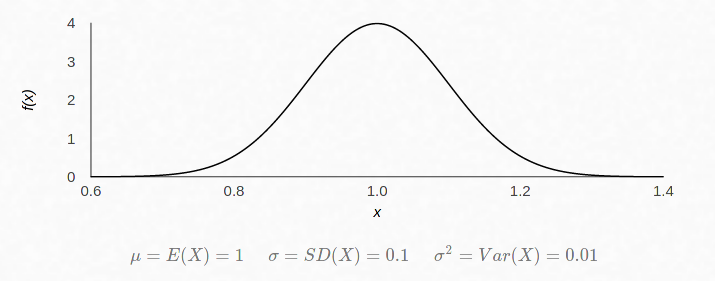
\includegraphics[width=0.5\linewidth]{normal_distribution}
        \caption{Normal distribution with $\mu = 1$ and $\sigma = 0.1$.}
    \end{figure}
    
    
    \subsection{NPC}\label{subsection:npc}
    Every NPC has his own \texttt{script} and a vector of \texttt{commodities}. Player can talk to NPC by selecting ``NPC: Talk to [\textit{NPC's name}]'' in actions menu, which calls NPC's virtual function \texttt{triggerEvent()}. 
    \par
    When \texttt{NPC}'s \texttt{triggerEvent()} is called, \texttt{NPC}'s \texttt{script} and a list of \texttt{commodities} will print out. \texttt{Player} can select the item he/she want to buy.
    \par
    Every commodity in \texttt{commodities} has the type \texttt{pair<int, Item>}, where \texttt{int} is the price of the item, and \texttt{Item} is the item to be sold. If \texttt{Player}'s \texttt{money} is larger than the price of the commodity, then he/she can buy the item. Otherwise, ``You don't have enough money!'' will print out.
    
    
    \subsection{Game Logic}
    In this project, game state is defined as a enum with three possible values: \textit{win}, \textit{lose}, or \textit{indeterminate}. When player is in the exit room, then the game state is \textit{win}. If player's $HP = 0$, then the game state is \textit{lose}. Otherwise, it is \textit{indeterminate}.
    
    \subsection{Record System} \label{subsection:record_system}
    The record system is implemented by saving/loading json file on disk. In fact, all game data can be represented as a \texttt{nlohmann::json}\footnote{\text{https://github.com/nlohmann/json}} object. The json file is highly human-readable and structurized, so the game can be customized easily. The map in this game can be changed by modifying \texttt{GAME\_DATA} in \texttt{Dungeon.cpp}, or simply editing the saved json file.
    \par
    Every class excluding \texttt{Dungeon} has its own \texttt{getJson()} method, which can return a \texttt{nlohmann::json} object. Game data is saved by subsequently calling \texttt{getJson()} of every class. Similarly, Every class excluding \texttt{Dungeon} has its own constructor that accepts \texttt{nlohmann::json} object as its parameter. Game data is loaded by subsequently calling constructor of every class.
    
    
    \subsection{Optional Enhancement}
    \begin{itemize}
        \item $LV$, $EXP$ System
        \begin{itemize}
            \item I added $LV$(level) and $EXP$(experience) system in this game. Player's health, attack and defense not only depends on his/her equipment, but also depends on his/her level. (See \ref{subsection:show_stats} for further detail.)
        \end{itemize}
        \item Enhanced Fighting System
        \begin{itemize}
            \item $ATK$/$DEF$ in this game are divided into two types: physical and magical. Different types of $ATK$ can deal different damage to monsters or player. Similarily, different types of $DEF$ can shield different types of $ATK$. (See \ref{subsection:fighting} for further detail.)
            \item When monsters died, their equipment will dropped onto the ground. Monsters' $EXP$ and $Money$ will also transfer to player. If player's $LV$ upgrades after defeating the monster, his/her HP will be refilled.
        \end{itemize}
        \item Equipment System
        \begin{itemize}
            \item Player can choose a variety of weapons and armors to prepare for different combat situation. For example, armors that can shield magical damage are good choices when attacking \textit{wizard} or \textit{magician}; weapons that has high physical damage are excellent choices when attacking monsters that are weak in physical defense.
            \item Furthermore, I divided items in this game into 7 categories:  \textit{Helmet}, \textit{Chestplate}, \textit{Leggings}, \textit{Boots}, \textit{Shield}, \textit{Weapon} and \textit{Usable}. Player can only equip one equipment of the same type (\textit{Usable} can only be used once).
        \end{itemize}
        \item Trading System
        \begin{itemize}
            \item I added $Money$ in this game, player can use money to trade with NPC. (See \ref{subsection:npc} for further detail.)
        \end{itemize}
        \item Customizable Game
        \begin{itemize}
            \item Game data is written in json file, so the game is highly customizable. (See \ref{subsection:record_system} for further detail.)
        \end{itemize}
        \item New Object: Chest
        \begin{itemize}
            \item I added chest in this game. When player opens a chest, then items in that chest can be picked up.
        \end{itemize}
        \item Use Smart Pointer to Prevent Memory Leak
        \begin{itemize}
            \item I used \texttt{shared\_ptr} extensively in this project. This smart pointer can avoid the problem of dangling pointer, so that memory leak would not occur.
        \end{itemize}
        \item Better Gaming Experience
        \begin{itemize}
            \item I've made a lot of optimization on the interface of the game to make the game more interesting. (See section \ref{subsection:results} for further detail.)
        \end{itemize}
        \item This Report XD
        \begin{itemize}
            \item I've made great effort on this report. To my mind, being able to describe how this game works is just as important as coding it.
        \end{itemize}
    \end{itemize}

\section{Results}\label{subsection:results}
\begin{figure}[H]
    \centering
    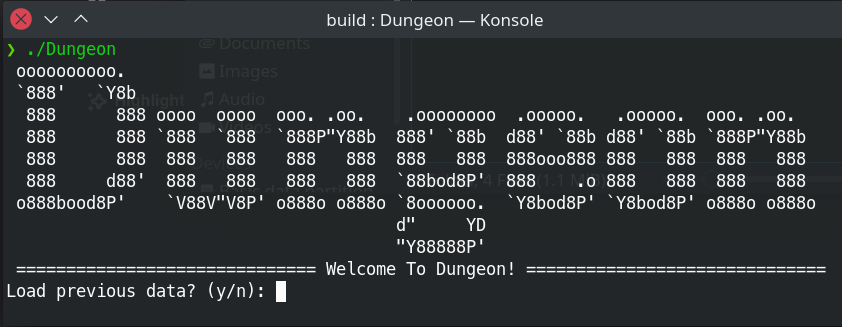
\includegraphics[width=0.7\linewidth]{welcome}
    \caption{welcome screen}
\end{figure}
\begin{figure}[H]
    \centering
    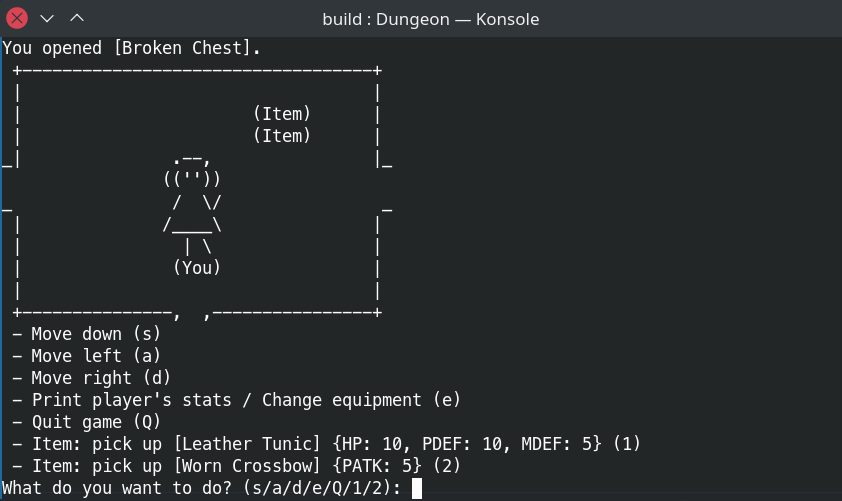
\includegraphics[width=0.7\linewidth]{actions_menu}
    \caption{actions menu / open chest / pick up items}
\end{figure}
\begin{figure}[H]
    \centering
    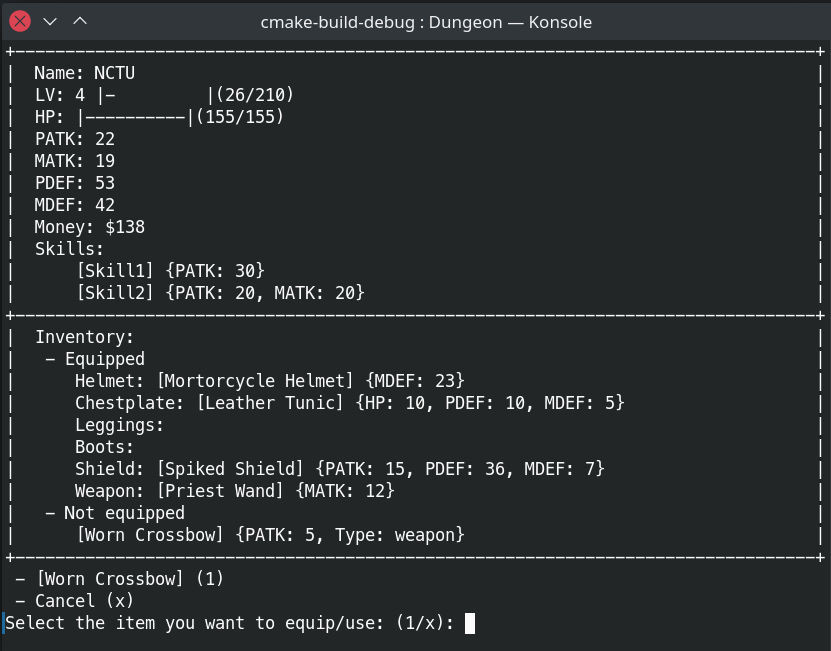
\includegraphics[width=0.7\linewidth]{print_stats}
    \caption{print player's stats / change equipment}
\end{figure}
\begin{figure}[H]
    \centering
    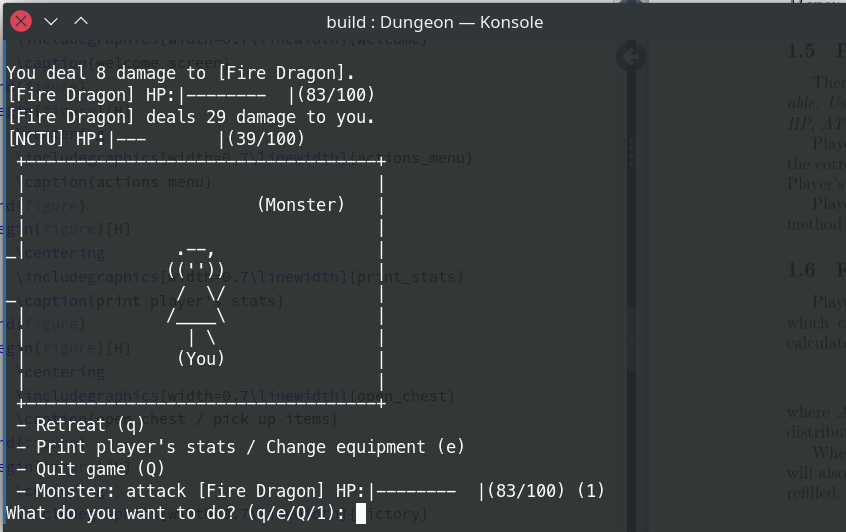
\includegraphics[width=0.7\linewidth]{fight}
    \caption{fight with monster}
\end{figure}
\begin{figure}[H]
    \centering
    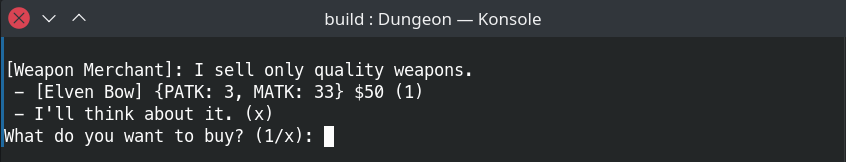
\includegraphics[width=0.7\linewidth]{talk_npc}
    \caption{talk to NPC}
\end{figure}
\begin{figure}[H]
    \centering
    
\includegraphics[width=0.7\linewidth]{victory}
    \caption{win}
\end{figure}
\begin{figure}[H]
    \centering
    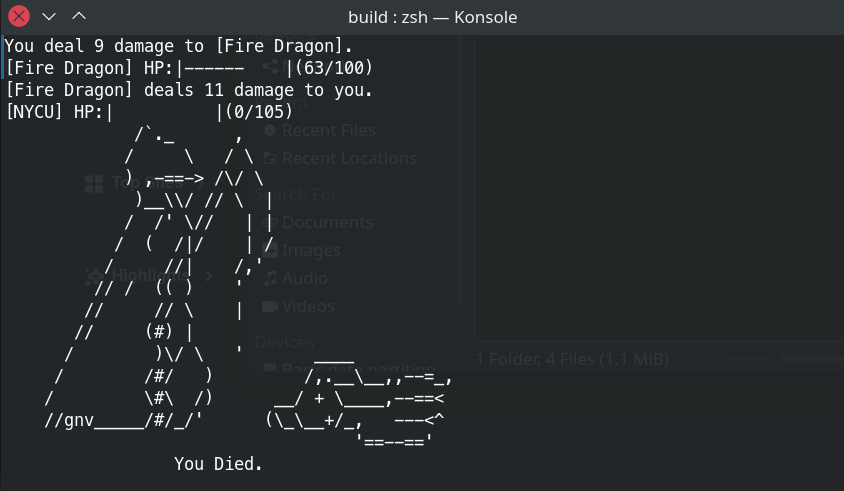
\includegraphics[width=0.7\linewidth]{lose}
    \caption{lose}
\end{figure}
    
\section{Discussion}

    In this section, I'll talk about some bad designs I've made in this project. Although these bad designs don't affect the functionality of the program, it can have great impact on extensibility and readability of the project. Therefore, I think it's necessary to record these mistakes, so that I can avoid these errors in the future.
    \subsection{the parameters in \texttt{triggerEvent()} should be modified}
    In this project, the function signature of \texttt{triggerEvent} is \texttt{triggerEvent(\textbf{Object\&})}. However, it seems that \texttt{triggerEvent(\textbf{Player\&})} would make more sense, since only \texttt{Player} can interact with \texttt{Object}. If \texttt{triggerEvent} accepts \texttt{Object\&} as its parameter, then it means that \texttt{Object} can interact with other \texttt{Object}, but I've not implemented this feature so far.
    \par
    Therefore, I think it's better to substitute \texttt{Object\&} with \texttt{Player\&} in \texttt{triggerEvent()}. However, it can lead to another problem - \textbf{circular dependency} - because \texttt{triggerEvent(Player\&)} is declared in \texttt{Object}, \texttt{Player} is also inherited from \texttt{Object}. Compile errors rises after I changed \texttt{Object\&} to \texttt{Player\&} in \texttt{triggerEvent()}'s parameter list.
    
    \subsection{Interactable objects should be distinguished from ordinary \texttt{Object}}
    In this game, \texttt{Room} has a member variable \texttt{objectPtrs}, which has the type \texttt{vector<shared\_ptr<Object>>} and it can store pointers of objects in that room. However, it's unreasonable to store \texttt{Player*} in \texttt{objectPtrs}, since there are only one \texttt{Player} in the game. However, it is allowed to do so, because \texttt{Player} is an \texttt{Object}. When a \texttt{Player*} is stored in \texttt{objectPtrs}, what should the program do when interacting with that \texttt{Player}? It's kind of weird to interact with other \texttt{Player} in a single-player game.
    \par
    Therefore, it think we should distinguish ordinary \texttt{Object} from interactable objects, i.e. \texttt{Chest}, \texttt{Item}, \texttt{Monster}, and \texttt{NPC}. Maybe we can create a new class named \texttt{InteractableObject}, and place \texttt{triggerEvent()} in it. \texttt{Chest}, \texttt{Item}, \texttt{Monster} and \texttt{NPC} are inherited from both \texttt{Object} and \texttt{InteractableObject} (by using multiple inheritance). In this way, the data type of \texttt{objectPtrs} can be changed to \texttt{vector<shared\_ptr<InteractableObject>>}, so \texttt{Player} would not be considered as an interactable object (because it is inherited only from \texttt{Object}).

\section{Conclusion}
This project was made possible thanks to various advantages of OOP principles. OOP allowed this project to become more concise, well-organized, and easy-to-read. On working with this project, I encounter many difficulties related to OOP. By tracing errors generated at compilation times, I learnt a lot when solving these problems. I'm sure that I become much more familiar with C++ after finishing this project.

\end{document}
